\documentclass{beamer}

%================= TIẾNG VIỆT =================
\usepackage[utf8]{inputenc}
\usepackage[T5]{fontenc}
\usepackage[vietnamese]{babel}

%================= GÓI TOÁN =================
\usepackage{amsmath, amssymb, bm}
\usepackage{graphicx}
\usepackage{hyperref}
\usepackage{multirow}
%================= THEME =================
\usetheme{Madrid}
\usefonttheme{professionalfonts}
\usefonttheme{serif}

% Bỏ thanh mục lục trên đầu và nút điều hướng
\setbeamertemplate{headline}{}
\setbeamertemplate{navigation symbols}{}
\setbeamertemplate{footline}[frame number]

%================= ĐỊNH NGHĨA =================
\def\bsmu{\bm{\mu}}
\def\bsx{\bm{x}}
\def\bsX{\bm{X}}
\def\R{\mathbb{R}}

\graphicspath{{Figures/}}

%================= THÔNG TIN =================
\title{Tiếp cận phương pháp LDA của R.A. Fisher \\
	trong phân loại mẫu thống kê}

\author{Phùng Ngọc Bảo -- 2212318}

\institute[]{
	\centering
	
\includegraphics[height=2.0cm]{LogoMathDLU} \\[0.3cm]
	Khoa Toán -- Tin học, Trường Đại học Đà Lạt \\[0.25cm]
	\textbf{Giảng viên hướng dẫn:} Đặng Phước Huy, Huỳnh Bảo Tuyên
}

\date{Ngày 2 tháng 6 năm 2026}

\begin{document}
	
	%================= SLIDE 1 =================
	\begin{frame}
		\titlepage
	\end{frame}
	
	%================= SLIDE 2 =================
	\begin{frame}{Mục tiêu của đề tài}
		\begin{itemize}
			\item Trình bày cơ sở lý thuyết của phương pháp LDA.
			\item Làm rõ ý tưởng hình học trong tiếp cận của Fisher.
			\item Xây dựng hàm phân biệt LDA theo lý thuyết Bayes.
			\item Chỉ ra sự tương đồng giữa hai cách tiếp cận.
			\item Minh họa phương pháp LDA của Fisher trên dữ liệu Iris và dữ liệu mô phỏng.
		\end{itemize}
	\end{frame}

	
	%================= SLIDE 3 =================
		\begin{frame}{Nội dung trình bày}
		\begin{enumerate}
			\item Giới thiệu bài toán phân loại mẫu thống kê.
			\item Tiếp cận LDA của Fisher.
			\item Tiếp cận LDA theo lý thuyết Bayes.
			\item Sự tương đương giữa Fisher và Bayes.
			\item Minh họa một chiều trên bộ dữ liệu Iris.
			\item Minh họa hai chiều trên dữ liệu mô phỏng.
			\item Kết luận và hướng phát triển.
		\end{enumerate}
	\end{frame}
	

%================= SLIDE 4 =================

\begin{frame}{Bài toán phân loại mẫu thống kê} \small Cho tập dữ liệu huấn luyện gồm \(n\) quan sát \[ \mathcal{D} = \{(\bsx_i,y_i): i=1,2,\ldots,n\}, \] trong đó \(\bsx_i \in \R^d\) là vectơ đặc trưng của quan sát thứ \(i\), còn \(y_i\) là nhãn lớp tương ứng. Giả sử bài toán có \(K\) lớp \[ C_1,C_2,\ldots,C_K, \] khi đó nhãn lớp thỏa mãn \[ y_i \in \{1,2,\ldots,K\}. \] Nếu \(y_i=k\), ta nói quan sát \(\bsx_i\) thuộc lớp \(C_k\). Với một quan sát mới \(\bsx\), mục tiêu là xây dựng quy tắc phân loại \[ \widehat{G}(\bsx)\in \{C_1,C_2,\ldots,C_K\}, \] sao cho quan sát mới được gán vào lớp phù hợp nhất. \begin{block}{Mục tiêu} Tìm một biên quyết định giúp phân tách các lớp trong không gian đặc trưng. \end{block} \end{frame}




%================= SLIDE 6 =================
\begin{frame}[t]{Tiếp cận Fisher: Ý tưởng hình học}
	\small
	
	\begin{block}{Câu hỏi của Fisher}
		Có thể tìm một hướng chiếu tuyến tính sao cho sau khi chiếu,
		hai lớp được tách biệt tốt nhất hay không?
	\end{block}
	
	\vspace{0.1cm}
	Một hướng chiếu tốt cần thỏa:
	\begin{itemize}
		\item Trung bình hai lớp sau chiếu cách xa nhau.
		\item Dữ liệu trong từng lớp sau chiếu có độ phân tán thấp.
	\end{itemize}
	
	\vfill
	
	\begin{figure}
		\centering
		
\includegraphics[width=0.54\textwidth]{image_1_Fisher_idea.png}
		
		\vspace{0.05cm}
		{\scriptsize Hình minh họa ý tưởng hình học của Fisher LDA, xem tài liệu \cite{hastie2009}.}
	\end{figure}
	
	\vfill
\end{frame}



	

%================= SLIDE 8 =================
\begin{frame}{Ma trận tán xạ giữa lớp và trong lớp}
	Xét bài toán phân loại hai lớp \(C_1\) và \(C_2\).
	Gọi \(\bm{\mu}_1,\bm{\mu}_2\) lần lượt là vectơ trung bình của hai lớp,
	còn \(\bm{\mu}\) là vectơ trung bình của toàn bộ dữ liệu.
	
	Ma trận tán xạ giữa hai lớp
	\[
	\Sigma_B
	=
	n_1(\bm{\mu}_1-\bm{\mu})(\bm{\mu}_1-\bm{\mu})^T
	+
	n_2(\bm{\mu}_2-\bm{\mu})(\bm{\mu}_2-\bm{\mu})^T.
	\]
	
	Ma trận tán xạ trong lớp
	\[
	\Sigma_W
	=
	\sum_{\bsx_i\in C_1}
	(\bsx_i-\bm{\mu}_1)(\bsx_i-\bm{\mu}_1)^T
	+
	\sum_{\bsx_i\in C_2}
	(\bsx_i-\bm{\mu}_2)(\bsx_i-\bm{\mu}_2)^T.
	\]
\end{frame}


	

%================= SLIDE 9 =================
\begin{frame}{Tiêu chuẩn Fisher}
	Trong trường hợp hai lớp, Fisher chiếu mỗi quan sát \(\bsx\in\R^d\) lên một trục có phương \(\bm{\beta}\)
	\[
	z=\bm{\beta}^T\bsx.
	\]
	
	Sau phép chiếu, mong muốn:
	\begin{itemize}
		\item Hai trung bình lớp cách xa nhau.
		\item Các điểm trong cùng một lớp ít phân tán.
	\end{itemize}
	
	Do đó, tiêu chuẩn Fisher được xác định bởi
	\[
	J(\bm{\beta})
	=
	\frac{\bm{\beta}^T\Sigma_B\bm{\beta}}
	{\bm{\beta}^T\Sigma_W\bm{\beta}}.
	\]
	
	\begin{block}{Bài toán tối ưu}
		Tìm hướng chiếu \(\bm{\beta}\neq \bm{0}\) sao cho
		\[
		\bm{\beta}_{\text{opt}}
		=
		\arg\max_{\bm{\beta}\neq \bm{0}}
		J(\bm{\beta}).
		\]
	\end{block}
\end{frame}


	

%================= SLIDE 10 =================
\begin{frame}{Liên hệ với thương Rayleigh}
	Từ tiêu chuẩn Fisher, ta cần giải bài toán tối ưu
	\begin{equation}
		\max_{\bm{\beta}\neq \bm{0}}
		J(\bm{\beta})
		=
		\max_{\bm{\beta}\neq \bm{0}}
		\frac{\bm{\beta}^T\Sigma_B\bm{\beta}}
		{\bm{\beta}^T\Sigma_W\bm{\beta}}.
		\tag{1}
	\end{equation}
	
	\(\Sigma_W\) là ma trận xác định dương. Đặt
	\begin{equation}
		\bm{y}=\Sigma_W^{1/2}\bm{\beta},
		\qquad
		\bm{\beta}=\Sigma_W^{-1/2}\bm{y}.
		\tag{2}
	\end{equation}
	
	Khi đó, tiêu chuẩn Fisher được đưa về dạng thương Rayleigh
	\begin{equation}
		J(\bm{\beta})
		=
		\frac{\bm{y}^T S\bm{y}}{\bm{y}^T\bm{y}},
		\qquad
		S=
		\Sigma_W^{-1/2}\Sigma_B\Sigma_W^{-1/2}.
		\tag{3}
	\end{equation}
	
	\begin{block}{Nhận xét}
		Cực đại của thương Rayleigh đạt tại vectơ riêng ứng với giá trị riêng lớn nhất của \(S\).
	\end{block}
\end{frame}


%================= SLIDE 11 =================
\begin{frame}{Nghiệm tối ưu Fisher}
	Từ bài toán tối ưu theo tiêu chuẩn Fisher và dạng thương Rayleigh, ta thu được phương chiếu tối ưu của Fisher
	\begin{equation}
		\bm{\beta}_{\text{opt}}
		\propto
		\Sigma_W^{-1}(\bm{\mu}_1-\bm{\mu}_2).
		\tag{4}
	\end{equation}
	
	Do phương chiếu không thay đổi khi nhân \(\bm{\beta}\) với một hằng số khác \(0\), ta thường chọn
	\begin{equation}
		\bm{\beta}_{\text{opt}}
		=
		\Sigma_W^{-1}(\bm{\mu}_1-\bm{\mu}_2).
		\tag{5}
	\end{equation}
	
	\begin{block}{Ý nghĩa}
		\(\bm{\beta}_{\text{opt}}\) là hướng chiếu làm tăng khoảng cách giữa hai lớp sau chiếu,
		đồng thời giảm độ phân tán trong từng lớp.
	\end{block}
\end{frame}


%================= SLIDE 12 =================
\begin{frame}{Biên phân loại theo Fisher}
	Sau khi xác định hướng chiếu tối ưu \(\bm{\beta}_{\text{opt}}\), mỗi quan sát \(\bsx\) được chiếu lên trục một chiều:
	\begin{equation}
		y=\bm{\beta}_{\text{opt}}^T\bsx.
		\tag{6}
	\end{equation}
	
	Trung bình của hai lớp sau chiếu là
	\[
	\bar{y}_k=\bm{\beta}_{\text{opt}}^T\bm{\mu}_k,
	\qquad k=1,2.
	\]
	
	Luật phân lớp theo Fisher được xác định bởi
	\begin{equation}
		\widehat{G}(\bsx)
		=
		\arg\min_{k=1,2}
		\left|y-\bar{y}_k\right|.
		\tag{7}
	\end{equation}
	
	Biên tách biệt là điểm có khoảng cách đến hai trung bình sau chiếu bằng nhau
	\begin{equation}
		\left|
		y_{\text{bnd}}-\bar{y}_1
		\right|
		=
		\left|
		y_{\text{bnd}}-\bar{y}_2
		\right|.
		\tag{8}
	\end{equation}
	
	\begin{block}{Phương trình biên} \begin{equation} \left[ \Sigma_W^{-1}(\bm{\mu}_1-\bm{\mu}_2) \right]^T \bsx_{\text{bnd}} - \frac{1}{2} \left( \bm{\mu}_1^T\Sigma_W^{-1}\bm{\mu}_1 - \bm{\mu}_2^T\Sigma_W^{-1}\bm{\mu}_2 \right) =0. \tag{9} \end{equation} \end{block}
\end{frame}

%================= SLIDE 13 =================
\begin{frame}{Tiếp cận Bayes trong phân loại}
	Giả sử với mỗi lớp \(C_k\), ta có
	\begin{equation}
		(\bsX\mid G=k) \sim f_k(\bsx),
		\qquad 
		P(G=k)=\pi_k,
		\quad k=1,2,\ldots,K.
		\tag{10}
	\end{equation}
	
	Theo quy tắc Bayes, với quan sát \(\bsx\), ta gán \(\bsx\) vào lớp có xác suất hậu nghiệm lớn nhất
	\begin{equation}
		G_B(\bsx)
		=
		\arg\max_{k}
		P(G=k\mid \bsX=\bsx).
		\tag{11}
	\end{equation}
	
	Theo công thức Bayes,
	\begin{equation}
		P(G=k\mid \bsX=\bsx)
		=
		\frac{\pi_k f_k(\bsx)}
		{\sum_{\ell=1}^{K}\pi_\ell f_\ell(\bsx)}
		\propto
		\pi_k f_k(\bsx).
		\tag{12}
	\end{equation}
	
	Quy tắc phân loại Bayes được viết gọn thành
	\begin{equation}
		G_B(\bsx)
		=
		\arg\max_{k}
		\left\{
		\pi_k f_k(\bsx)
		\right\}.
		\tag{13}
	\end{equation}
\end{frame}

%================= SLIDE 14 =================
\begin{frame}{Mô hình Gauss và hàm tách biệt}
	\small
	
	Giả sử hai lớp có phân phối chuẩn nhiều chiều với cùng ma trận hiệp phương sai
	\begin{equation}
		(\mathbf{X}\mid G=k)
		\sim
		N_d(\bm{\mu}_k,\Sigma),
		\qquad
		P(G=k)=\pi_k,
		\quad k=1,2.
		\tag{14}
	\end{equation}
	
	Khi đó, mật độ điều kiện trên từng lớp là
	\begin{equation}
		f_k(\bsx)
		=
		\frac{1}{(2\pi)^{d/2}|\Sigma|^{1/2}}
		\exp
		\left\{
		-\frac{1}{2}
		(\bsx-\bm{\mu}_k)^T
		\Sigma^{-1}
		(\bsx-\bm{\mu}_k)
		\right\}.
		\tag{15}
	\end{equation}
	
	Từ quy tắc Bayes, hàm tách biệt Bayes
	\begin{equation}
		\delta_k(\bsx)
		=
		-\frac{1}{2}\ln|\Sigma|
		-\frac{1}{2}
		(\bsx-\bm{\mu}_k)^T
		\Sigma^{-1}
		(\bsx-\bm{\mu}_k)
		+\ln\pi_k.
		\tag{16}
	\end{equation}
	
	Hàm tách biệt rút gọn thành
	\begin{equation}
		\delta_k(\bsx)
		=
		\bsx^T\Sigma^{-1}\bm{\mu}_k
		-
		\frac{1}{2}
		\bm{\mu}_k^T\Sigma^{-1}\bm{\mu}_k
		+
		\ln\pi_k.
		\tag{17}
	\end{equation}
\end{frame}

%================= SLIDE 16 =================
\begin{frame}{Biên quyết định Bayes hai lớp}
	\small
	
	Trong bài toán hai lớp, biên quyết định Bayes được xác định bởi
	\[
	\delta_1(\bsx)=\delta_2(\bsx). \tag{18}
	\]
	
	Từ hàm phân biệt rút gọn, ta thu được
	\[
	\bsx^T\Sigma^{-1}(\bm{\mu}_1-\bm{\mu}_2)
	-\frac{1}{2}
	\left(
	\bm{\mu}_1^T\Sigma^{-1}\bm{\mu}_1
	-
	\bm{\mu}_2^T\Sigma^{-1}\bm{\mu}_2
	\right)
	+
	\ln\frac{\pi_1}{\pi_2}
	=0. \tag{19}
	\]
	
	Nếu \(\pi_1=\pi_2\), thì \(\ln\dfrac{\pi_1}{\pi_2}=0\).
	
	Trong thực nghiệm
	\[
	\pi_k \approx \widehat{\pi}_k,\qquad
	\bm{\mu}_k \approx \widehat{\bm{\mu}}_k,\qquad
	\Sigma \approx \widehat{\Sigma}.
	\]
	
	\begin{block}{Biên quyết định thực nghiệm khi \(\widehat{\pi}_1=\widehat{\pi}_2\)}
		\[
		\bsx^T\widehat{\Sigma}^{-1}
		(\widehat{\bm{\mu}}_1-\widehat{\bm{\mu}}_2)
		-
		\frac{1}{2}
		\left(
		\widehat{\bm{\mu}}_1^T\widehat{\Sigma}^{-1}\widehat{\bm{\mu}}_1
		-
		\widehat{\bm{\mu}}_2^T\widehat{\Sigma}^{-1}\widehat{\bm{\mu}}_2
		\right)
		=0. \tag{20}
		\]
	\end{block}
\end{frame}



%================= SLIDE 17 =================
\begin{frame}{Đánh giá kết quả phân loại}
	\small
	
	Với hàm tổn thất \(0-1\), phân loại đúng có chi phí \(0\), phân loại sai có chi phí \(1\).
	Kết quả phân loại được tổng hợp bằng ma trận lỗi:
	
	\vspace{0.15cm}
	\begin{table}
		\centering
		\renewcommand{\arraystretch}{1.25}
		\begin{tabular}{|c|cc|c|}
			\hline
			\multirow{2}{*}{Các lớp dự báo} 
			& \multicolumn{2}{c|}{Các lớp đúng} 
			& \multirow{2}{*}{Tổng cộng} \\ 
			\cline{2-3}
			& \(C_1\) & \(C_2\) & \\ 
			\hline
			\(\widehat{C}_1\) & \(n_{11}\) & \(n_{12}\) & \(n_{1\bullet}\) \\
			\(\widehat{C}_2\) & \(n_{21}\) & \(n_{22}\) & \(n_{2\bullet}\) \\
			\hline
			Tổng cộng & \(n_{\bullet 1}\) & \(n_{\bullet 2}\) & \(n\) \\
			\hline
		\end{tabular}
	\end{table}
	
Trong đó, \(n_{ij}\) là số quan sát được dự báo vào lớp \(\widehat{C}_i\) và thực tế thuộc lớp \(C_j\).

\vspace{0.1cm}
\[
\mathrm{Overall\ Accuracy}
=
\frac{n_{11}+n_{22}}{n},
\qquad
\mathrm{TPM}
=
\frac{n_{12}+n_{21}}{n}.
\]

\[
\underbrace{
	P(\widehat{C}_j\mid C_j)
	=
	\frac{n_{jj}}{n_{\bullet j}}
}_{\text{Recall của lớp } C_j},
\qquad
\underbrace{
	P(C_j\mid \widehat{C}_j)
	=
	\frac{n_{jj}}{n_{j\bullet}}
}_{\text{Precision của lớp } C_j},
\quad j=1,2.
\]
\end{frame}


%================= SLIDE 18 =================
\begin{frame}{Giới thiệu bộ dữ liệu Iris}
	\small
	
	Bộ dữ liệu Iris gồm \(150\) quan sát, chia đều cho \(3\) lớp hoa:
	\[
	C_1=\textit{setosa},\qquad
	C_2=\textit{versicolor},\qquad
	C_3=\textit{virginica}.
	\]
	
	Mỗi quan sát có \(4\) thuộc tính:
	\[
	\text{Sepal.Length},\quad
	\text{Sepal.Width},\quad
	\text{Petal.Length},\quad
	\text{Petal.Width}.
	\]
	
	\vspace{0.1cm}
	\begin{center}
		\renewcommand{\arraystretch}{1.15}
		\begin{tabular}{|c|c|c|c|c|c|}
			\hline
			STT & Sepal.L & Sepal.W & Petal.L & Petal.W & Species \\ \hline
			1 & 5.1 & 3.5 & 1.4 & 0.2 & setosa \\ 
			2 & 4.9 & 3.0 & 1.4 & 0.2 & setosa \\ 
			3 & 4.7 & 3.2 & 1.3 & 0.2 & setosa \\ 
			4 & 4.6 & 3.1 & 1.5 & 0.2 & setosa \\ 
			5 & 5.0 & 3.6 & 1.4 & 0.2 & setosa \\ \hline
		\end{tabular}
	\end{center}
	
	Trong đồ án, bộ dữ liệu này được dùng để minh họa quy tắc phân loại một chiều bằng LDA.
\end{frame}

%================= SLIDE 18 =================
\begin{frame}{Minh họa phân loại 1 chiều: Versicolor và Virginica}
	\small
	
	Xét thuộc tính \textit{Petal.Length} với hai lớp
	\[
	C_1=\textit{versicolor},\qquad C_2=\textit{virginica}.
	\]
	
	Từ dữ liệu Iris, ta có
	\[
	n_1=n_2=50,\qquad \widehat{\pi}_1=\widehat{\pi}_2=\frac{1}{2}.
	\]
	
	Trung bình mẫu và phương sai mẫu của hai lớp là
	\[
	\widehat{\mu}_1=4{,}260\ \text{cm},\quad s_1^2=0{,}2208\ \text{cm}^2,
	\qquad
	\widehat{\mu}_2=5{,}552\ \text{cm},\quad s_2^2=0{,}3046\ \text{cm}^2.
	\]
	
	Phương sai mẫu gộp:
	\[
	s_p^2
	=
	\frac{(n_1-1)s_1^2+(n_2-1)s_2^2}{n_1+n_2-2}
	=
	\frac{49(0{,}2208)+49(0{,}3046)}{98}
	\approx 0{,}2627\ \text{cm}^2.
	\]
	
	Vì \(\widehat{\pi}_1=\widehat{\pi}_2\), ngưỡng LDA là trung điểm hai trung bình:
	\[
	x_{\text{bnd}}
	=
	\frac{\widehat{\mu}_1+\widehat{\mu}_2}{2}
	=
	\frac{4{,}260+5{,}552}{2}
	=
	4{,}906\ \text{cm}.
	\]
	
	\[
	\widehat{G}(x)
	=
	\begin{cases}
		C_1, & x\le 4{,}906\ \text{cm},\\
		C_2, & x>4{,}906\ \text{cm}.
	\end{cases}
	\]
\end{frame}


	

%================= SLIDE 19 =================
\begin{frame}[t]{Minh họa phân loại 1 chiều: Versicolor và Virginica}
	\scriptsize
	\setlength{\abovedisplayskip}{3pt}
	\setlength{\belowdisplayskip}{3pt}
	
	\begin{columns}[T,totalwidth=\textwidth]
		
		%---------- CỘT TRÁI: HÌNH + MA TRẬN LỖI ----------
		\begin{column}{0.58\textwidth}
			\centering
			
			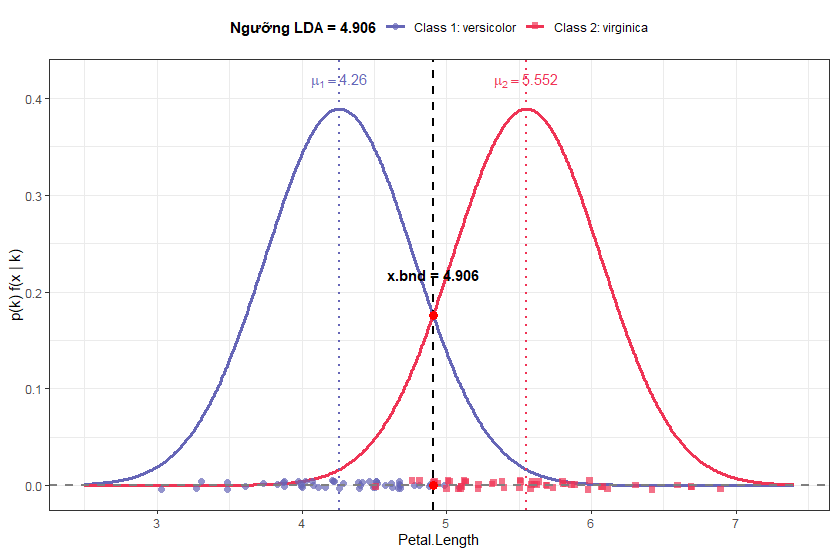
\includegraphics[width=\textwidth]{minh_họa_phân_phối_iris_versicolor_và_virginica.png}
			
			\vspace{0.08cm}
			Hai lớp có vùng chồng lấn quanh ngưỡng
			\[
			x_{\text{bnd}}=4{,}906\ \text{cm}.
			\]
			
			\vspace{0.05cm}
			\textbf{Ma trận lỗi}
			\[
			\begin{array}{c|cc}
				& C_1 & C_2 \\ \hline
				\widehat{C}_1 & 48 & 6 \\
				\widehat{C}_2 & 2 & 44
			\end{array}
			\]
		\end{column}
		
		%---------- CỘT PHẢI: CHỈ SỐ ĐÁNH GIÁ ----------
		\begin{column}{0.39\textwidth}
			\textbf{Tỷ lệ phân loại lỗi}
			\[
			\mathrm{TPM}
			=
			\frac{6+2}{100}
			=
			0{,}08
			=
			8\%.
			\]
			
			\vspace{0.15cm}
			\textbf{Độ chính xác tổng thể}
			\[
			\mathrm{Overall\ Accuracy}
			=
			1-\mathrm{TPM}
			=
			92\%.
			\]
			
			\vspace{0.22cm}
\[
\begin{array}{c|cc}
	& \text{precision} & \text{recall} \\ \hline
	C_1 & 88{,}89\% & 96\% \\
	C_2 & 95{,}65\% & 88\%
\end{array}
\]
		\end{column}
		
	\end{columns}
\end{frame}




%================= SLIDE 20 =================
\begin{frame}{Minh họa phân loại 1 chiều: Setosa và Versicolor}
	\small
	
	Xét thuộc tính \textit{Petal.Length} với hai lớp
	\[
	C_1=\textit{setosa},\qquad C_2=\textit{versicolor}.
	\]
	
	Từ dữ liệu Iris, ta có
	\[
	n_1=n_2=50,\qquad \widehat{\pi}_1=\widehat{\pi}_2=\frac{1}{2}.
	\]
	
	Trung bình mẫu và phương sai mẫu của hai lớp là
	\[
	\widehat{\mu}_1=1{,}462\ \text{cm},\quad s_1^2=0{,}0302\ \text{cm}^2,
	\qquad
	\widehat{\mu}_2=4{,}260\ \text{cm},\quad s_2^2=0{,}2208\ \text{cm}^2.
	\]
	
	Phương sai mẫu gộp:
	\[
	s_p^2
	=
	\frac{49(0{,}0302)+49(0{,}2208)}{98}
	\approx
	0{,}1255\ \text{cm}^2.
	\]
	
	Vì \(\widehat{\pi}_1=\widehat{\pi}_2\), ngưỡng LDA là
	\[
	x_{\text{bnd}}
	=
	\frac{1{,}462+4{,}260}{2}
	=
	2{,}861\ \text{cm}.
	\]
	
\end{frame}


%================= SLIDE 21 =================
\begin{frame}[t]{Minh họa phân loại 1 chiều: Setosa và Versicolor}
	\scriptsize
	\setlength{\abovedisplayskip}{3pt}
	\setlength{\belowdisplayskip}{3pt}
	
	\begin{columns}[T,totalwidth=\textwidth]
		
		%---------- CỘT TRÁI: HÌNH + MA TRẬN LỖI ----------
		\begin{column}{0.58\textwidth}
			\centering
			
			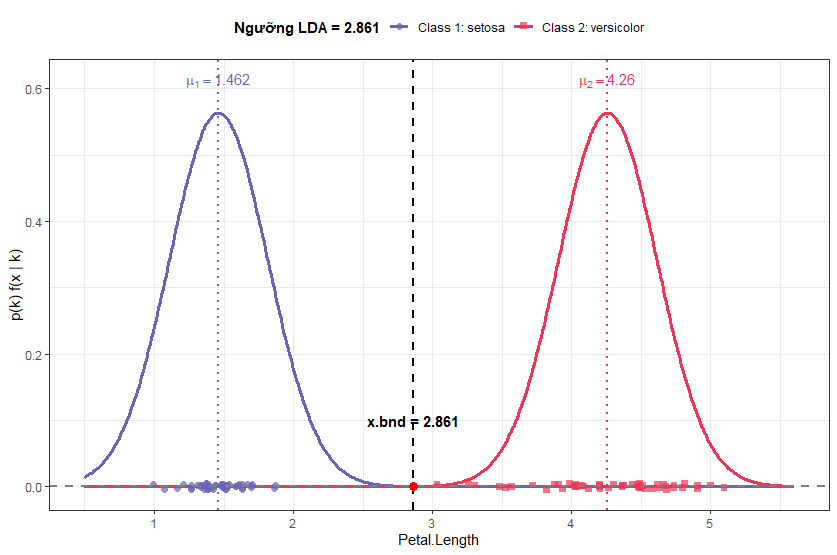
\includegraphics[width=\textwidth]{bayes1Dgood.png}
			
			\vspace{0.08cm}
			Hai lớp tách biệt hoàn toàn theo \textit{Petal.Length};
			\[
			x_{\text{bnd}}=2{,}861\ \text{cm}.
			\]
			
			Trong dữ liệu thực tế:
			\[
			\max(\textit{setosa})=1{,}9\ \text{cm},
			\qquad
			\min(\textit{versicolor})=3{,}0\ \text{cm}.
			\]
			
			Do đó, ngưỡng LDA nằm trong khoảng trống giữa hai lớp.
			
		\end{column}
		
		%---------- CỘT PHẢI: ĐÁNH GIÁ ----------
		\begin{column}{0.39\textwidth}
			
			\vspace{0.05cm}
			\textbf{Ma trận lỗi}
			\[
			\begin{array}{c|cc}
				& C_1 & C_2 \\ \hline
				\widehat{C}_1 & 50 & 0 \\
				\widehat{C}_2 & 0 & 50
			\end{array}
			\]
			\textbf{Tỷ lệ phân loại lỗi}
			\[
			\mathrm{TPM}=0\%.
			\]
			
			\vspace{0.18cm}
			\textbf{Độ chính xác tổng thể}
			\[
			\mathrm{Accuracy}=100\%.
			\]
			
			\vspace{0.22cm}

			\[
			\begin{array}{c|cc}
				& \text{precision} & \text{recall} \\ \hline
				C_1 & 100\% & 100\% \\
				C_2 & 100\% & 100\%
			\end{array}
			\]
		\end{column}
		
	\end{columns}
\end{frame}
	
%================= SLIDE 22 =================
\begin{frame}{Mô phỏng hai chiều: Hai lớp ít chồng lấn}
	\scriptsize
	\setlength{\abovedisplayskip}{3pt}
	\setlength{\belowdisplayskip}{3pt}
	
	\textbf{1. Thiết lập mô phỏng}
	\[
	n_1=n_2=500,\qquad
	\bm{\mu}_1=
	\begin{pmatrix}
		3\\
		3
	\end{pmatrix},
	\qquad
	\bm{\mu}_2=
	\begin{pmatrix}
		4\\
		4
	\end{pmatrix},
	\qquad
	\Sigma=
	\begin{pmatrix}
		2 & -1{,}5\\
		-1{,}5 & 2
	\end{pmatrix}.
	\]
	
	\textbf{2. Biên LDA lý thuyết}
	\[
	\bm{\beta}_{\text{opt}}
	=
	\Sigma^{-1}(\bm{\mu}_1-\bm{\mu}_2)
	=
	\begin{pmatrix}
		-2\\
		-2
	\end{pmatrix},
	\qquad
	\frac{\bm{\mu}_1+\bm{\mu}_2}{2}
	=
	\begin{pmatrix}
		3{,}5\\
		3{,}5
	\end{pmatrix}.
	\]
	\[
	\bm{\beta}_{\text{opt}}^T
	\left(
	\bm{x}_{\text{bnd}}
	-
	\frac{\bm{\mu}_1+\bm{\mu}_2}{2}
	\right)
	=0
	\quad \Rightarrow \quad
	-2x_1-2x_2+14=0
	\]
	\[
	\Rightarrow \quad
	\boxed{x_2=7-x_1}.
	\]
	
	\textbf{3. Biên LDA thực nghiệm từ dữ liệu mẫu}
	\[
	\widehat{\bm{\mu}}_1=
	\begin{pmatrix}
		3{,}0345\\
		2{,}9611
	\end{pmatrix},
	\quad
	\widehat{\bm{\mu}}_2=
	\begin{pmatrix}
		4{,}0687\\
		3{,}9000
	\end{pmatrix},
	\quad
	\widehat{\Sigma}=
	\begin{pmatrix}
		2{,}2449 & -1{,}7388\\
		-1{,}7388 & 2{,}2465
	\end{pmatrix}.
	\]
	\[
	\bm{b}_{\text{opt}}
	=
	\widehat{\Sigma}^{-1}
	(\widehat{\bm{\mu}}_1-\widehat{\bm{\mu}}_2)
	=
	\begin{pmatrix}
		-1{,}9587\\
		-1{,}9340
	\end{pmatrix}.
	\]
	\[
	\bm{b}_{\text{opt}}^T
	\left(
	\bm{x}_{\text{bnd}}
	-
	\frac{\widehat{\bm{\mu}}_1+\widehat{\bm{\mu}}_2}{2}
	\right)
	=0
	\quad \Rightarrow \quad
	-1{,}9587x_1-1{,}9340x_2+13{,}5912=0
	\]
	\[
	\Rightarrow \quad
	\boxed{x_2=7{,}0276-1{,}0128x_1}.
	\]
\end{frame}


%================= SLIDE 23 =================
\begin{frame}[t]{Mô phỏng hai chiều: Hai lớp ít chồng lấn}
	\scriptsize
	\setlength{\abovedisplayskip}{3pt}
	\setlength{\belowdisplayskip}{3pt}
	
	\begin{columns}[T,totalwidth=\textwidth]
		
		%---------- CỘT TRÁI: HÌNH PHÂN LỚP ----------
		\begin{column}{0.55\textwidth}
			\centering
			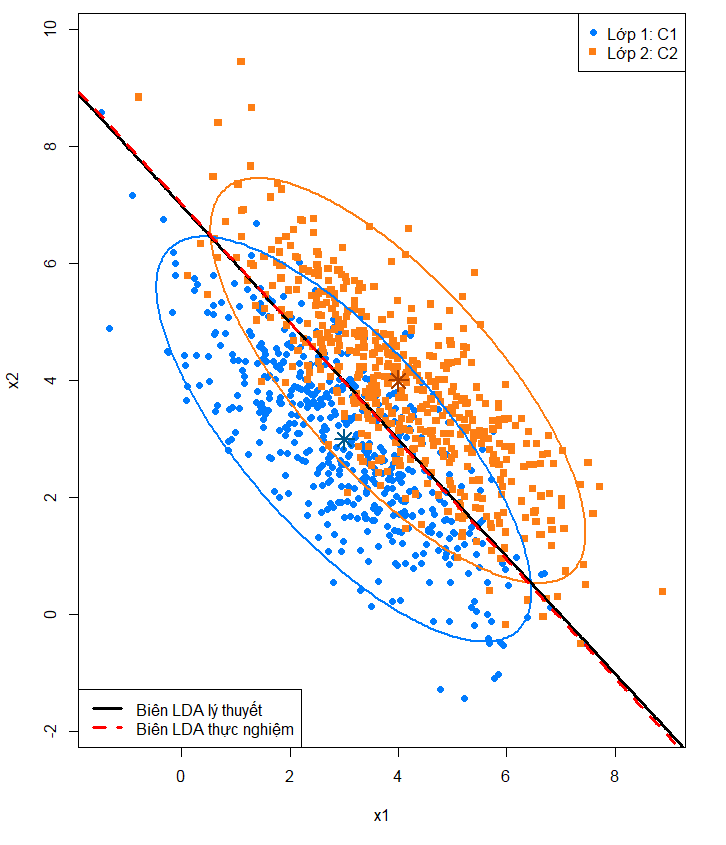
\includegraphics[width=\textwidth]{normal_dis_2_classes_test.png}
			
			\vspace{0.08cm}
		\end{column}
		
		%---------- CỘT PHẢI: MA TRẬN LỖI + ĐÁNH GIÁ ----------
		\begin{column}{0.42\textwidth}
			\centering
			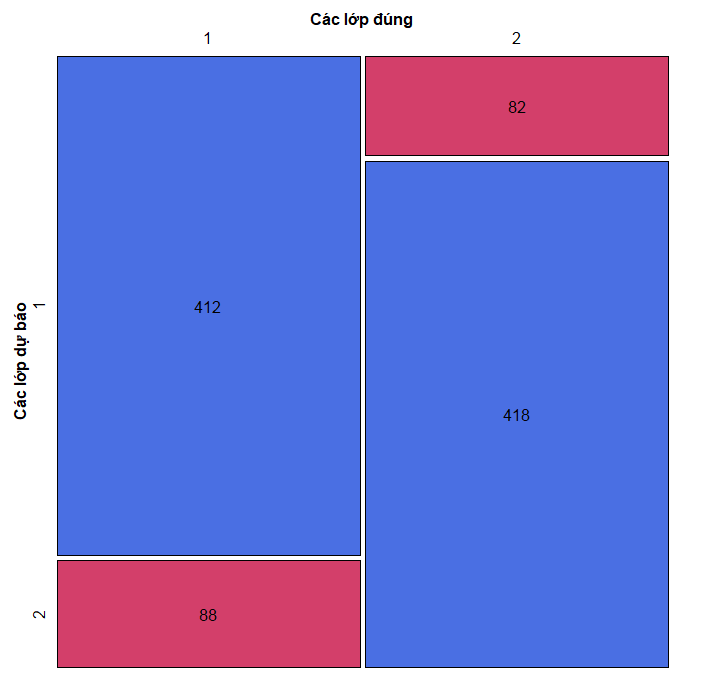
\includegraphics[width=1\textwidth]{confusion_matrix_test.png}
			
			\vspace{0.08cm}
			\textbf{Kết quả đánh giá}
	
			\[
			\widehat{\mathrm{TPM}}
			=
			17{,}0\%,
			\qquad
			\mathrm{Accuracy}
			=
			83{,}0\%.
			\]
			\[
			\begin{array}{c|cc}
				& \text{precision} & \text{recall} \\ \hline
				C_1 & 83{,}40\% & 82{,}40\% \\
				C_2 & 82{,}61\% & 83{,}60\%
			\end{array}
			\]
		\end{column}
		
	\end{columns}
\end{frame}


%================= SLIDE 24 =================
\begin{frame}{Mô phỏng hai chiều: Hai lớp chồng lấn nhiều}
	\scriptsize
	\setlength{\abovedisplayskip}{3pt}
	\setlength{\belowdisplayskip}{3pt}
	
	\textbf{1. Thiết lập mô phỏng}
	\[
	n_1=n_2=500,\qquad
	\bm{\mu}_1=
	\begin{pmatrix}
		3\\
		3
	\end{pmatrix},
	\qquad
	\bm{\mu}_2=
	\begin{pmatrix}
		3{,}2\\
		2{,}5
	\end{pmatrix},
	\qquad
	\Sigma=
	\begin{pmatrix}
		2 & 1\\
		1 & 2
	\end{pmatrix}.
	\]
	
	\textbf{2. Biên LDA lý thuyết}
	\[
	\bm{\beta}_{\text{opt}}
	=
	\Sigma^{-1}(\bm{\mu}_1-\bm{\mu}_2)
	=
	\begin{pmatrix}
		-0{,}3\\
		0{,}4
	\end{pmatrix},
	\qquad
	\frac{\bm{\mu}_1+\bm{\mu}_2}{2}
	=
	\begin{pmatrix}
		3{,}1\\
		2{,}75
	\end{pmatrix}.
	\]
	\[
	\bm{\beta}_{\text{opt}}^T
	\left(
	\bm{x}_{\text{bnd}}
	-
	\frac{\bm{\mu}_1+\bm{\mu}_2}{2}
	\right)
	=0
	\quad \Rightarrow \quad
	-0{,}3x_1+0{,}4x_2-0{,}17=0
	\]
	\[
	\Rightarrow \quad
	\boxed{x_2=0{,}425+0{,}75x_1}.
	\]
	
	\textbf{3. Biên LDA thực nghiệm từ dữ liệu mẫu}
	\[
	\widehat{\bm{\mu}}_1=
	\begin{pmatrix}
		2{,}9716\\
		3{,}0225
	\end{pmatrix},
	\quad
	\widehat{\bm{\mu}}_2=
	\begin{pmatrix}
		3{,}2101\\
		2{,}5101
	\end{pmatrix},
	\quad
	\widehat{\Sigma}=
	\begin{pmatrix}
		1{,}9507 & 0{,}8710\\
		0{,}8710 & 1{,}9595
	\end{pmatrix}.
	\]
	\[
	\bm{b}_{\text{opt}}
	=
	\widehat{\Sigma}^{-1}
	(\widehat{\bm{\mu}}_1-\widehat{\bm{\mu}}_2)
	=
	\begin{pmatrix}
		-0{,}2982\\
		0{,}3940
	\end{pmatrix}.
	\]
	\[
	\bm{b}_{\text{opt}}^T
	\left(
	\bm{x}_{\text{bnd}}
	-
	\frac{\widehat{\bm{\mu}}_1+\widehat{\bm{\mu}}_2}{2}
	\right)
	=0
	\quad \Rightarrow \quad
	-0{,}2982x_1+0{,}3940x_2-0{,}1684=0
	\]
	\[
	\Rightarrow \quad
	\boxed{x_2=0{,}4274+0{,}7567x_1}.
	\]
\end{frame}


%================= SLIDE 25 =================
\begin{frame}[t]{Mô phỏng hai chiều: Hai lớp chồng lấn nhiều}
	\scriptsize
	\setlength{\abovedisplayskip}{3pt}
	\setlength{\belowdisplayskip}{3pt}
	
	\begin{columns}[T,totalwidth=\textwidth]
		
		\begin{column}{0.55\textwidth}
			\centering
			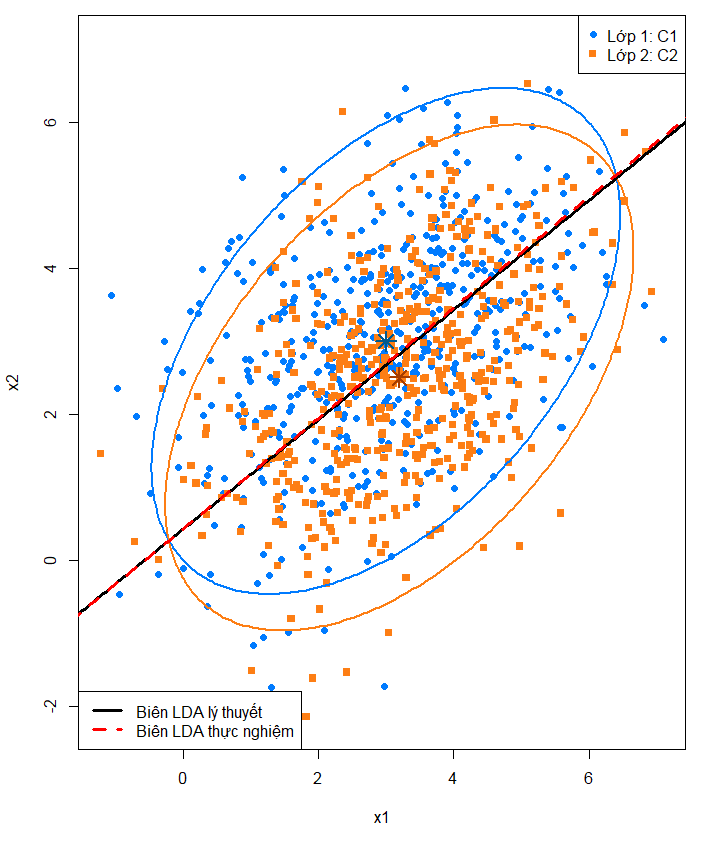
\includegraphics[width=\textwidth]{normal_dis_2_classes_overlap_test.png}
			
			\vspace{0.08cm}
		\end{column}
		
		\begin{column}{0.42\textwidth}
			\centering
			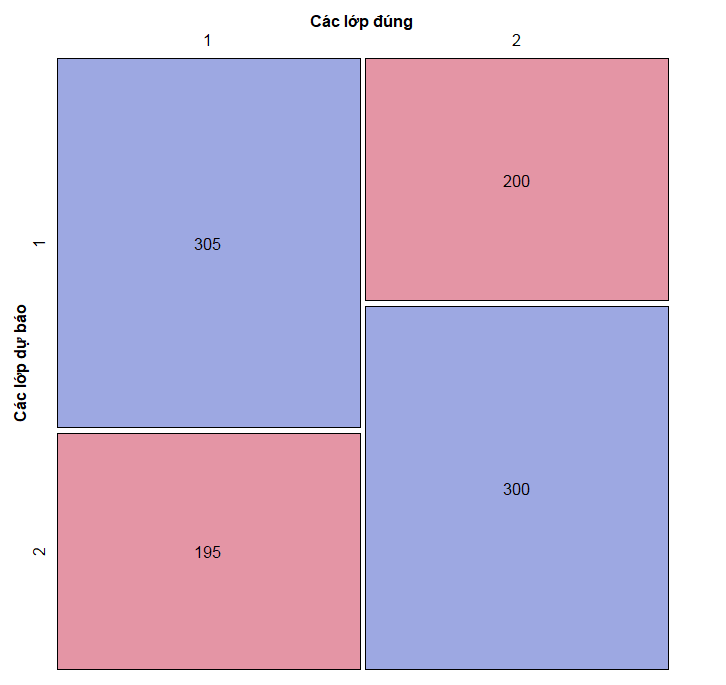
\includegraphics[width=1\textwidth]{confusion_matrix_overlap_test.png}
			
			\vspace{0.08cm}
			\textbf{Kết quả đánh giá}
			\[
			\widehat{\mathrm{TPM}}=39{,}5\%,
			\qquad
			\mathrm{Accuracy}=60{,}5\%.
			\]
			
			\[
			\begin{array}{c|cc}
				& \text{precision} & \text{recall} \\ \hline
				C_1 & 60{,}40\% & 61{,}0\% \\
				C_2 & 60{,}61\% & 60{,}0\%
			\end{array}
			\]
		\end{column}
		
	\end{columns}
\end{frame}


%================= SLIDE 26 =================
\begin{frame}{Mô phỏng hai chiều: Hai lớp tách biệt hoàn toàn}
	\scriptsize
	\setlength{\abovedisplayskip}{3pt}
	\setlength{\belowdisplayskip}{3pt}
	
	\textbf{1. Thiết lập mô phỏng}
	\[
	n_1=n_2=500,\qquad
	\bm{\mu}_1=
	\begin{pmatrix}
		3\\
		3
	\end{pmatrix},
	\qquad
	\bm{\mu}_2=
	\begin{pmatrix}
		13\\
		3
	\end{pmatrix},
	\qquad
	\Sigma=
	\begin{pmatrix}
		2 & 0\\
		0 & 2
	\end{pmatrix}.
	\]
	
	\textbf{2. Biên LDA lý thuyết}
	\begin{columns}[T]
		\begin{column}{0.5\textwidth}
			Vì \(\Sigma=2I\), hai lớp có cùng phương sai theo hai hướng và không tương quan. Biên LDA lý thuyết là đường trung trực của đoạn nối hai tâm:
			\[
			\bm{\beta}_{\text{opt}} = \begin{pmatrix} -5\\ 0 \end{pmatrix}, \quad
			\frac{\bm{\mu}_1+\bm{\mu}_2}{2} = \begin{pmatrix} 8\\ 3 \end{pmatrix}.
			\]
		\end{column}
		\begin{column}{0.5\textwidth}
			Áp dụng công thức đường biên:
			\[
			\bm{\beta}_{\text{opt}}^T
			\left(
			\bm{x}_{\text{bnd}} - \frac{\bm{\mu}_1+\bm{\mu}_2}{2}
			\right)
			=0
			\]
			\[
			\Rightarrow \quad -5x_1+40=0 \quad \Rightarrow \quad \boxed{x_1=8}.
			\]
		\end{column}
	\end{columns}
	
	\vspace{2mm} % Thêm khoảng trắng nhỏ giữa 2 phần cho thoáng
\textbf{3. Biên LDA thực nghiệm từ dữ liệu mẫu}
\begin{columns}[T]
	\begin{column}{0.5\textwidth}
		\[
		\widehat{\bm{\mu}}_1=
		\begin{pmatrix}
			2{,}9491\\
			2{,}9966
		\end{pmatrix},
		\quad
		\widehat{\bm{\mu}}_2=
		\begin{pmatrix}
			12{,}9999\\
			3{,}0117
		\end{pmatrix}
		\]
		\[
		\widehat{\Sigma}=
		\begin{pmatrix}
			2{,}1682 & -0{,}0051\\
			-0{,}0051 & 1{,}8841
		\end{pmatrix}.
		\]
	\end{column}
	\begin{column}{0.5\textwidth}
		\[
		\bm{b}_{\text{opt}}
		=
		\begin{pmatrix}
			-4{,}6356\\
			-0{,}0205
		\end{pmatrix}.
		\]
		\[
		\bm{b}_{\text{opt}}^T
		\left(
		\bm{x}_{\text{bnd}}
		-
		\frac{\widehat{\bm{\mu}}_1+\widehat{\bm{\mu}}_2}{2}
		\right)
		=0
		\]
		\[
		\Rightarrow \quad -4{,}6356x_1-0{,}0205x_2+37{,}0283=0.
		\]
		Vì hệ số của \(x_2\) rất nhỏ nên biên thực nghiệm gần như là đường thẳng đứng:
		\[
		\Rightarrow \quad
		\boxed{x_1\approx 7{,}9878}.
		\]
	\end{column}
\end{columns}
\end{frame}

%================= SLIDE 27 =================
\begin{frame}[t]{Mô phỏng hai chiều: Hai lớp tách biệt hoàn toàn}
	\scriptsize
	\setlength{\abovedisplayskip}{3pt}
	\setlength{\belowdisplayskip}{3pt}
	
	\begin{columns}[T,totalwidth=\textwidth]
		
		%---------- CỘT TRÁI: HÌNH PHÂN LỚP ----------
		\begin{column}{0.55\textwidth}
			\centering
			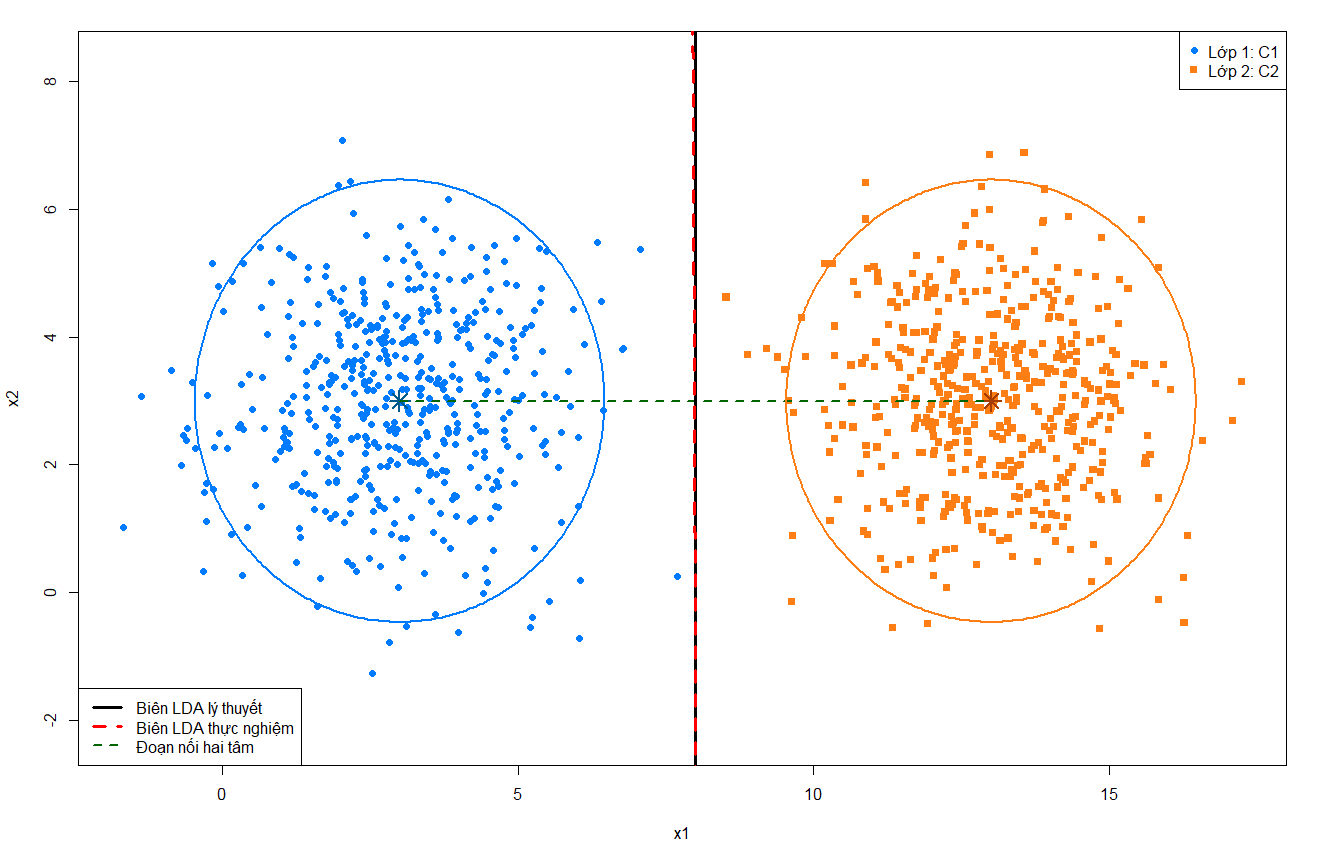
\includegraphics[width=\textwidth]{circular_separable_2_classes.png}
			
			\vspace{0.08cm}
			{\scriptsize Hai lớp tách biệt rõ ràng; biên LDA gần với đường trung trực của hai tâm.}
		\end{column}
		
		%---------- CỘT PHẢI: MA TRẬN LỖI + ĐÁNH GIÁ ----------
		\begin{column}{0.42\textwidth}
			\centering
			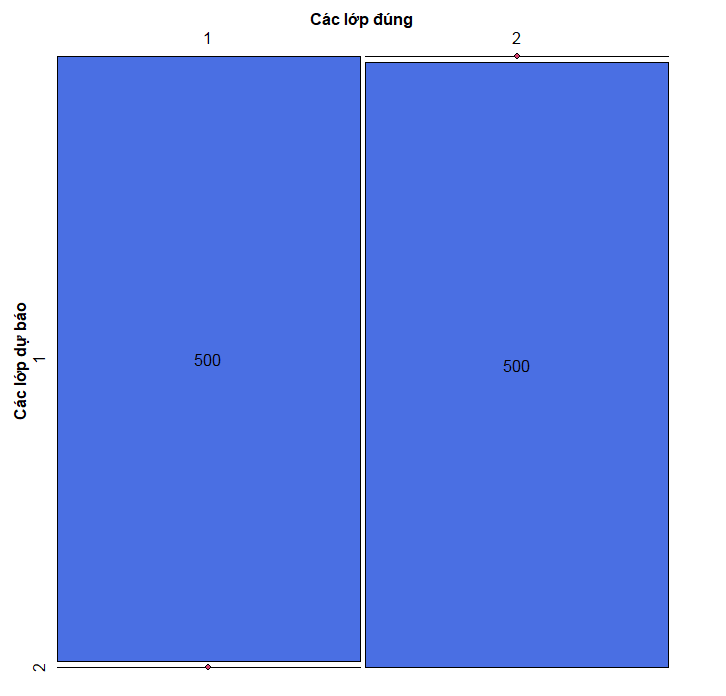
\includegraphics[width=1\textwidth]{confusion_matrix_separable_test.png}
			
			\vspace{0.08cm}
			\textbf{Kết quả đánh giá}
			\[
			\widehat{\mathrm{TPM}}=0\%,
			\qquad
			\mathrm{Accuracy}=100\%.
			\]
			
			\[
			\begin{array}{c|cc}
				& \text{precision} & \text{recall} \\ \hline
				C_1 & 100\% & 100\% \\
				C_2 & 100\% & 100\%
			\end{array}
			\]
			
			\vspace{0.12cm}

		\end{column}
		
	\end{columns}
\end{frame}
	
	%================= SLIDE 25 =================
	\begin{frame}{Kết luận và hướng phát triển}
		\textbf{Kết quả đạt được}
		\begin{itemize}
			\item Trình bày được cơ sở lý thuyết của Fisher LDA.
			\item Chứng minh phương chiếu tối ưu trong trường hợp hai lớp.
			\item Làm rõ sự tương đồng giữa Fisher LDA và Bayes LDA.
			\item Minh họa bằng dữ liệu Iris và dữ liệu mô phỏng hai chiều cho phân loại hai lớp.
		\end{itemize}
		
		\textbf{Hướng phát triển}
		\begin{itemize}
			\item Mở rộng LDA cho bài toán nhiều lớp.
			\item So sánh LDA với các phương pháp phân loại mẫu thống kê khác.
		\end{itemize}
	\end{frame}
	
	%================= SLIDE 26 =================
%================= SLIDE TÀI LIỆU THAM KHẢO =================
\begin{frame}{Tài liệu tham khảo}
	\scriptsize
	
	\begin{thebibliography}{99}
		
		\bibitem{dang2010}
		Đặng Phước Huy,
		\textit{Bài giảng tóm tắt -- Thống kê toán học},
		Trường Đại học Đà Lạt, 2010.
		
		\bibitem{dang2023}
		Đặng Phước Huy,
		\textit{Bài giảng tóm tắt -- Phân tích thống kê nhiều chiều},
		Trường Đại học Đà Lạt, 2023.
		
		\bibitem{dang2025}
		Đặng Phước Huy,
		\textit{Bài giảng tóm tắt -- Lý thuyết học thống kê},
		Trường Đại học Đà Lạt, 2025.
		
		\bibitem{le2022}
		Lê Đình Phú,
		\textit{Suy diễn thống kê với phương pháp mẫu nhỏ},
		Khóa luận tốt nghiệp cử nhân toán học,
		Khoa Toán -- Tin học, Trường Đại học Đà Lạt, 2022.
		
		\bibitem{fisher1936}
		R. A. Fisher,
		\textit{The Use of Multiple Measurements in Taxonomic Problems},
		Annals of Eugenics, Vol. 7, No. 2, pp. 179--188, 1936.
		
		\bibitem{bishop2006}
		Christopher M. Bishop,
		\textit{Pattern Recognition and Machine Learning},
		Springer, 2006.
		
		\bibitem{hastie2009}
		Trevor Hastie, Robert Tibshirani, Jerome Friedman,
		\textit{The Elements of Statistical Learning: Data Mining, Inference, and Prediction},
		2nd ed., Springer, 2009.
		
		\bibitem{johnson2007}
		Johnson R. A., Wichern D. W.,
		\textit{Applied Multivariate Statistical Analysis},
		Pearson Prentice Hall, Pearson Education, Inc, 2007.
		
		\bibitem{iris1936}
		R. A. Fisher,
		\textit{Iris},
		UCI Machine Learning Repository, 1936.
		DOI: \url{https://doi.org/10.24432/C56C76}.
		
	\end{thebibliography}
	
\end{frame}
	
	%================= SLIDE 27 =================
	\begin{frame}
		\centering
		\vspace{1.5cm}
		{\Large \textbf{Cảm ơn thầy cô và các bạn đã lắng nghe!}}
	\end{frame}
	
\end{document}